\documentclass{myproc}
\usepackage{mydef,myenv}
\usepackage{times,mathptm}
\usepackage[all]{xypic}
%\usepackage{MinionPro}
\usepackage{graphicx}
\usepackage{alltt}
\usepackage[T1]{fontenc}
\DeclareGraphicsExtensions{.png,.jpg}

\usepackage{hyperref}
\hypersetup{
    colorlinks, 
    citecolor=black, 
    filecolor=black, 
    linkcolor=blue, 
    urlcolor=black
}

\begin{document}
\small

\setlength\oddsidemargin{-1.2cm}
\setlength\evensidemargin{-0.5cm}
\setlength\textwidth{19cm}
\addtolength\topmargin{-1cm}
\addtolength\textheight{-0.5cm}

\title{\textcolor{red2}{\large\bf Relevant Technologies}}
%\author{\normalsize{}Cheoljoo Jeong}
\date{\normalsize\today}
\maketitle

\tableofcontents

%% \section{TRENDS}
%% \subsection{Maker movement -- Manufacturing barrier collapses}

%% \subsection{IoT (Internet of Things)}
%% \bit
%% \w F.~daCosta.
%% \newblock {\em Rethinking the Internet of Things: A Scalable Approach to
%%   Connecting Everything}.
%% \newblock Apress, Inc., 2013.

%% \eit

%% \subsection{M2M (Machine-to-Machine)}

%% \subsection{Industrial Internet -- Initiative by GE}

%% \subsection{Service Web 3.0 -- Initiative by EU}

%% \subsection{Rise of robots}

%% \subsection{Autonomous cars}

%% \subsection{SOA (Service-Oriented Architecture)}

%%%%
%%%%
%%%%
\section{COMPUTER SCIENCE IN GENERAL}
\bit
\w R.~L. Ashenhurst, editor.
\newblock {\em ACM Turing Award Lectures: The First Twenty Years: 1966 to
  1985}.
\newblock ACM Press Anthology Series. ACM Press, 1987.

\w C. A. R. Hoare et al. Grand Challenges in Computing.
\eit

\section{ALGORITHMS AND THEORY OF COMPUTATION}
\subsection{General Textbooks}
\bit
\w T.~H. Cormen, C.~E. Leiserson, R.~L. Rivest, and C.~Stein.
\newblock {\em Introduction to Algorithms}.
\newblock MIT Press, Cambridge, MA, second edition, 2001.
\w M.~R. Garey and M.~S. Johnson.
\newblock {\em Computers and Intractability: A Guide to the Theory of
  {NP}-Completeness}.
\newblock W. H. Freeman, 1979.
\eit

\subsection{Complexity Theories}
\bit
\w E.~Kushilevitz.
\newblock Communication complexity.
\newblock Manuscript, 1996.
\eit


\subsection{Distributed Algorithms}
\bit
\w N.~Lynch.
\newblock {\em Distributed Algorithms}.
\newblock Morgan Kaufmann Publishers, San Francisco, CA, 1996.

\w H.~Attiya.
\newblock {\em Lecture Notes for Course \#236357: Distributed Algorithms}.
\newblock Department of Computer Science, The Technion, Haifa, January 1994.

\w D.~Karger, E.~Lehman, T.~Leighton, M.~Levine, D.~Lewin, and R.~Panigrahy.
\newblock Consistent hashing and random trees: Distributed caching protocols
  for relieving hot spots on the world wide web.
\newblock In {\em Proceedings of the 29th Annual ACM Symposium on Theory of
  Computing}, pages 654--663, 1997.
\eit

\section{PROGRAMMING LANGUAGES AND COMPILERS}
\subsection{General Textbooks}
\bit
\w \textcolor{blue2}{H.~Abelson, G.~J. Sussman, and J.~Sussman.
\newblock {\em Structure and Interpretation of Computer Programs}.
\newblock MIT Press, second edition, 1996.}

\w D.~P. Friedman, M.~Wand, and C.~T. Haynes.
\newblock {\em Essentials of Programming Languages}.
\newblock MIT Press, Cambridge, Massachusetts, 1992.

\w J.~C. Mitchell.
\newblock {\em Concepts in Programming Languages}.
\newblock Cambridge University Press, Cambridge, UK, 2003.

\w A.~V. Aho, M.~Lam, R.~Sethi, and J.~D. Ullman.
\newblock {\em Compilers: Principles, Techniques, and Tools}.
\newblock Addison-Wesley, second edition, 2006.

\w A.~Appel.
\newblock {\em Modern Compiler Implementation in ML}.
\newblock Cambridge University Press, Cambridge, UK, 1998.
\eit

\begin{figure*}[hbt]
\centerline{\includegraphics[width=16cm]{pics/prog-paradigms}}
\caption{Programming Paradigms}
\end{figure*}

\subsection{Functional Programming Languages}
\bit
\w D.~P. Friedman and M.~Wand.
\newblock Reification: Reflection without metaphysics.
\newblock In {\em Proceedings of LFP'~84, ACM SIGPLAN Conference on LISP and
  Functional Programming}, pages 348--355, 1984.

\w A.~Appel and T.~Jim.
\newblock Continuation-passing, closure-passing style.
\newblock In {\em Proceedings of POPL'~89, 16th Annual ACM Symposium on
  Principles of Programming Languages}, pages 293--302, 1989.

\w A.~Appel.
\newblock {\em Compiling with Continuations}.
\newblock Cambridge University Press, 1992.

\w A.~Appel.
\newblock {SSA} is functional.
\newblock {\em SIGPLAN Notices}, 1998.
\eit

\subsubsection{Racket}

\subsection{Object-oriented Programming Languages}
\bit
\w M.~Abadi and L.~Cardelli.
\newblock {\em A Theory of Objects}.
\newblock Springer Verlag, New York, NY, 1996.

\eit

\subsection{Logic Programming Languages}
\bit
\w Warren abstract machine
\w J.~L. Bates and R.~L. Constable.
\newblock Proofs as programs.
\newblock {\em ACM Transactions on Programming Languages and Systems},
  7(1):113--136, January 1985.
\eit

\subsection{Distributed Programming Languages}
\subsubsection{dRuby}
\subsubsection{Scala}
\bit
\w Scala $\equiv$ ``scalable language''
\w functional JVM language (i.e. interpreter written with Java)
  \bit
  \w allows easy stealing of Java classes into Scala (also, tons of Java-based libraries}
  \w {\em also, this is its weakness -- it's tied to Java}
  \eit
\w ``tastefully-typed'': statically-typed with type inference
\w \bb{mixin}: class which contains a combination of methods from other
classes -- ``interface with implemented methods''
\w \bb{actor}:
\begin{alltt}
  actor \{
    var sum = 0
    loop \{
      \textcolor{blue2}{// every actor has a {\em mailbox\/} in}
      \textcolor{blue2}{// which incoming messages are queued}
      receive \{
        case \bb{Data(bytes)}
          => sum += hash(bytes)
        \textcolor{blue2}{// send = "recipient ! msg"}
        case \bb{GetSum(requester)}
          => requester ! sum
      \}
    \}
  \}
\end{alltt}
\eit
\subsubsection{Erlang}
\bit
\w \bb{basics}
\bit
  \w world is concurrent: or {\em full of concurrent ``processes''}
  \w {\em message passing\/} is good: processes actually don't share data --
  \textcolor{red2}{shmem-based concurrency is difficult since maintaining
    data consistency is difficult esp. in presence of failures/delays}
  \w \textcolor{red2}{\textbf{COMMENT: message passing-based code is difficult
  to develop; how about letting users to shmem but we internally change it to
  message passing -- i.e. PROTOCOL SYNTHESIS + COMMUNICATOR GENERATOR}}
  \w target of {\em message delivery\/}: \bb{local process}, \bb{remote process}
  \w constructs for embracing \bb{failures}
  \w constructs for receptive code
\eit
\w \bb{three primitives for message-passing processes}
  \bit
  \w \bb{spawn}: \verb+Pid = spawn(Fun)+: create a process which executes
  function \verb+Fun+
  \w \bb{send} (\verb+Pid ! Message+): sends a message to the \bb{mailbox} of
  process \verb+Pid+
  \w \bb{receive}: remove a message from the \bb{mailbox} of the process which
  executes this ``receive''
     \begin{verbatim}
  receive
    Pattern1 [when Guard1] ->
      Expressions1;
    Pattern2 [when Guard2] ->
      Expressions2;
    ...
  end
     \end{verbatim}
  \eit
\w \bb{message passing}
  \bit
  \w \bb{simple message passing}
  \[
  \xymatrix@-1.5pc{
     \txt{\tt{}B!{self(),foo}} \\
   *++[o][F]\txt{A} \ar[rr]^{\{A, foo\}} & &
     *++[o][F]\txt{B} \\ 
  &&
  }
  \]
  \begin{verbatim}
                receive
                 {From,Msg} -> Actions
                end
  \end{verbatim}

  \w \bb{selective message reception}: pattern matched
  \[
  \xymatrix@-1.5pc{
   \txt{\tt{}C!foo} &&\\
     *++[o][F]\txt{A} \ar[rrd]^{foo} & & \\ 
            &&*++[o][F]\txt{C}\\
     *++[o][F]\txt{B} \ar[rru]_{bar} & & \\ 
     \txt{\tt{}C!bar} &&\\
  }\]
\begin{verbatim}
     receive foo -> true end,
     receive bar -> true end
\end{verbatim}
  \w \bb{selective message reception}: pattern matched
  \[
  \xymatrix@-1.5pc{
   \txt{\tt{}C!foo} &&\\
     *++[o][F]\txt{A} \ar[rrd]^{foo} & & \\ 
            &&*++[o][F]\txt{C}\\
     *++[o][F]\txt{B} \ar[rru]_{bar} & & \\ 
     \txt{\tt{}C!bar} &&\\
  }\]
\begin{verbatim}
     receive Msg
\end{verbatim}
  \eit
  
\w \textcolor{blue2}{\bb{distributed Erlang}}
  \bit
  \w \bb{Erlang node}
  \w \bb{name server}: 
  \eit
\eit
\subsubsection{Groovy}
\subsubsection{Ambit}
\subsubsection{Linda}


\subsection{Formal Semantics Of Programming Languages}
\bit
\w J.~Stoy.
\newblock {\em Denotational Semantics: The Scott-Stratchey Approach to
  Programming Language Theory}.
\newblock MIT Press, Cambridge, MA, 1977.

\w S.~Abramsky and A.~Jung.
\newblock Domain theory.
\newblock In S.~Abramsky, D.~M. Gabbay, and T.~S.~E. Maibaum, editors, {\em
  Handbook of Logic in Computer Science}, volume III, pages 1--168. Clarendon
  Press, 1991.

\eit

\subsection{Practices in Programming Languages}
\bit
\w G.~L. {Steele, Jr.}
\newblock Growing a language.
\newblock Talk given at OOPSLA'98, 1998.
\eit


\section{FORMAL METHODS}
\subsection{Process Algebras}
\subsubsection{General textbooks}
\bit
\w \textcolor{blue2}{H.~Bowman and R.~Gomez.
\newblock {\em Concurrency Theory: Calculi and Automata for Modelling Untimed
  and Timed Concurrent Systems}.
\newblock Springer Verlag, 2006.}
\eit
\subsubsection{CSP (Communicating Sequential Processes)}
\bit
\w C.~A.~R. Hoare.
\newblock {\em Communicating Sequential Processes}.
\newblock Prentice-Hall International, 1985.

\w S.~D. Brookes, C.~A.~R. Hoare, and A.~W. Roscoe.
\newblock A theory of communicating sequential processes.
\newblock {\em Journal of the ACM}, 31(3):560--599, 1984.
\eit


\subsubsection{CCS (Calculus of Communicating Systems)}
\bit
\w R.~Milner.
\newblock {\em A Calculus of Communicating Systems}.
\newblock Number~92 in Lecture Notes in Computer Science. Springer Verlag,
  1980.

\w M.~Hennessy and R.~Milner.
\newblock Algebraic laws for nondeterminism and concurrency.
\newblock {\em Journal of the ACM}, 32:137--161, 1985.

\w R.~Milner.
\newblock {\em Communication and Concurrency}.
\newblock Prentice Hall, 1989.

\w R.~Milner.
\newblock Semantics of concurrent processes.
\newblock In J.~van Leeuwen, editor, {\em Formal Models and Semantics},
  volume~B of {\em Handbook of Theoretical Computer Science}, pages 1201--1242.
  MIT Press, 1990.

\eit

\subsubsection{$\pi$-calculus}
\bit
\w R.~Milner.
\newblock {\em Communicating and Mobile Systems: The $\pi$-calculus}.
\newblock Cambridge University Press, Cambridge, UK, 1999.

\w R.~Milner.
\newblock Functions as processes.
\newblock {\em Mathematical Structures in Computer Science}, 2:119--141, 1992.

\w R.~Milner, J.~Parrow, and D.~Walker.
\newblock A calculus of mobile processes, part {I}.
\newblock {\em Information and Computation}, 100(1):1--40, September 1992.

\w R.~Milner, J.~Parrow, and D.~Walker.
\newblock A calculus of mobile processes, part {I}{I}.
\newblock {\em Information and Computation}, 100(1):41--77, September 1992.

\w R.~Milner.
\newblock {\em The Space and Motion of Communicating Agents}.
\newblock Cambridge University Press, 2009.

\w B.~Pierce. 
\newblock The Pict Programming Language. 
\eit

\subsection{Petri Nets}
\bit
\w T.~Murata.
\newblock Petri nets: Properties, analysis and applications.
\newblock {\em Proceedings of The IEEE}, 77(4):541--580, April 1989.
\eit

\bit
\w Each place represents one device. Token sync means ``join''. 1-1 mapping to
``fork-join''.
\eit


\subsection{Dataflow Process Networks}
\bit
\w \bb{Classification}
  \bit
  \w {Data-driven vs demand-driven}
  \w {Static vs dynamic}
  \eit
\w \bb{Example networks}
  \bit
 \w {Kahn network}
  \w {Synchronous network by Ed. Lee}
  \w {Dataflow machine by Arvind}
 \eit
\eit
\bit
\w G.~Kahn.
\newblock The semantics of a simple language for parallel programming.
\newblock In {\em Proceedings of the IFIP Congress 74}, 1974.

\w E.~A. Lee and T.~M. Parks.
\newblock Dataflow process networks.
\newblock {\em Proceedings of the IEEE}, 83(5):773--801, May 1995.
\eit

\subsection{\textcolor{red2}{\bf{}Modeling of Reactive Systems}}
\bit
\w D.~Harel.
\newblock Statecharts: A visual formalism for complex systems.
\newblock {\em Science of Computer Programming}, 8:231--274, 1987.

\w Reactive system modeling
\eit

\subsection{Modal and Temporal Logics}
\bit
\w Z.~Manna and A.~Pnueli.
\newblock {\em The Temporal Logic of Reactive and Concurrent Systems:
  Specification}.
\newblock Springer Verlag, 1991.
\eit

\subsection{Formal Verification}
\subsubsection{Model checking}
\subsubsection{Theorem proving}

\subsection{\textcolor{red2}{\bf{}Protocol Synthesis}}
\subsubsection{LOTOS}
\bit
\w ISO8807.
\newblock Information processing systems -- open systems interconnection --
  {L}{O}{T}{O}{S} -- a formal description technique based on the temporal
  ordering of observational behavior.
\newblock ISO 8807: 1989 (E), February 1989.

\w 
J.~A. Manas and T.~de~Miguel.
\newblock From {L}{O}{T}{O}{S} to {C}.
\newblock In K.~Turner, editor, {\em Proceedings of the 1st International
  Conference on Formal Description Technique (FORTE'88)}. North-Holland, 1988.

\eit


\subsubsection{SDL}
\subsection{Protocol synthesis}
\bit
\w \textcolor{blue2}{G.~J. Holzmann.
\newblock {\em Design and Validation of Computer Protocols}, chapter 10.
  Protocol Synthesis.
\newblock Prentice Hall, 1990.}
\eit


\section{OPERATING SYSTEMS}

\subsection{Operating Systems Practices}
\bit
\w D.~P. Bovet and M.~Cesati.
\newblock {\em Understanding the Linux Kernel}.
\newblock O'Reilly, third edition, 2006.
\eit

\section{COMPUTER NETWORKS}
\subsection{General Textbooks}
\bit
\w \textcolor{blue2}{L.~L. Peterson and B.~S. Davie.
\newblock {\em Computer Networks: A Systems Approach}.
\newblock Morgan Kaufmann Publishers, second edition, 2000.}
\eit

\subsection{Wireless Protocols}
\subsubsection{802.15.4}
\bit
\w physical and data link layer
\eit

\subsubsection{ZigBee}
\bit
\w network and application layer protocols on top of 802.15.4
\eit




\section{DISTRIBUTED COMPUTING}
\subsection{General Textbooks}
\bit
\w J.~Saltzer and M.~F. Kaashoek.
\newblock {\em Principles of Computer System Design: An Introduction}.
\newblock Morgan Kaufmann Publishers, 2009.

\w S.~Mullender, editor.
\newblock {\em Distributed Systems}.
\newblock Addison-Wesley, 2nd edition, 1993.

\w M.~Raynal.
\newblock {\em Distributed Algorithms for Message-Passing Systems}.
\newblock Springer Verlag, 2013.

\eit

\subsection{Theoretical Foundations}
\subsubsection{Synchronization models}
\bit
\w D.~Gelernter.
\newblock Generative communication in {Linda}.
\newblock {\em ACM Transactions on Programming Languages and Systems},
7(1):80--112, January 1985. 

\eit


\subsubsection{Remote procedure calls}
\bit
\w A.~D. Birrell and B.~J. Nelson.
\newblock Implementing remote procedure calls.
\newblock {\em ACM Transactions on Computer Systems}, 2(1):39--59, February
  1984.

\w A.~Birrell, G.~Nelson, S.~Owicki, and E.~Wobber.
\newblock Network objects.
\newblock SRC Research Report 115, Digital Equipment Corporation, 1994.

\w M.~Henning.
\newblock The rise and fall of {CORBA}.
\newblock {\em ACM Queue}, pages 28--34, June 2006.
\eit

\subsubsection{Synchronizers}
\bit
\w B.~Awerbuch.
\newblock Complexity of network synchronization.
\newblock {\em Journal of the ACM}, 32(4):804--823, October 1985.
\eit

\subsubsection{Logical clocks and clock synchronization}
\bit
\w L.~Lamport.
\newblock Time, clocks, and the ordering of events in a distributed system.
\newblock {\em Communications of the ACM}, 21(7):558--565, July 1978.
\eit

\subsubsection{Authentication}
\bit
\w B.~W. Lampson, M.~Abadi, M.~Burrows, and E.~Wobber.
\newblock Authentication in distributed systems: Theory and practice.
\newblock {\em ACM Transactions on Computer Systems}, 10(4):265--310, 1992.
\eit

\subsubsection{Scheduling}
\bit
\w M. Isard, V.~Prabhakaran, J.~Currey, U.~Wieder, K.~Talwar, and A.~Goldberg.
\newblock Quincy: Fair scheduling for distributed computing clusters.
\newblock In {\em Proceedings of the 22nd Symposium on Operating System
  Principles (SOSP'09)}, pages 261--276, 2009.
\eit

\subsubsection{Distributed lookup}
\bit
\w \bb{center al coordinator}: Napster, GFS
\w \bb{flooding}: send queries to a large set of machines -- Gnutella
\w \bb{DHT (distributed hash table}: Chord, CAN, Tapestry, Amazon Dynamo
\eit

\subsection{Practical Issues}
\subsubsection{\textcolor{red2}{\bf{}UUID: Universally Unique ID}}


\subsection{Naming and Directory Services}
\subsubsection{LDAP}
\subsubsection{JNDI (Java Naming \& Directory Interface)}
\bit
\w Usage \#1: lookup
   \begin{verbatim}
  printer = 
    (Printer) bldg7.lookup("puffin");
  printer.print(document);
\end{verbatim}
\w Usage \#2: get attributes
  \begin{verbatim}
  String[] attrs = 
    {"workphone", "cellphone"};
  boolsphons = 
    directory.getAttributes(
     "cn=bob o=sales c=US"/*key*/, 
     attrs);
 \end{verbatim}
\w Usage \#3: directory search
  \begin{verbatim}
  bobs = directory.search("cn=bob");
\end{verbatim}
\w \bb{existing naming services}: {\bf LDAP, DNS, NDS, ...}
\w \bb{Naming system}: has following components
   \bit
   \w \bb{naming scheme} (or naming convention): simple names, compound
   (hierarchical) names
   \w \bb{context}: an object whose state is a set of bindings (from name to ``object'') with distinct atomic names
     \bit
     \w provides \bb{lookup (resolution)} operation that returns an object,
     and may provide operations such as for \bb{binding} names,
     \bb{unbinding} names,  \bb{listing} bound names
     \w \bb{subcontext}: an atomic name in a context can be bound to another
     context object, say \bb{subcontext}, giving rise to compound names
     \eit
   \w \bb{naming system}: a connected set of contexts of the same type
   (i.e. have the same naming convention and provides the same set of
   operations with the same semantics)
   \w \bb{namespace}: the set of all names in a naming system
   \w \bb{composite name}: a name that spans multiple naming systems
      e.g. http://plato.mv.com/home/cjeong combines the DNS naming system
      (plato.mv.com) and  filesystem naming system
   \w {\em every name is interpreted relative to some context}
   \eit
\w \bb{directory objects}
\bit
\w  primary function of naming system: \bb{mapping names to objects} 
  \bit
  \w object can be any final atomic object or a directory object
  \eit
\w directory object can have attributes, etc.
\eit

\w \bb{JNDI API}
\bit
\w \bb{javax.naming}:
\w \bb{javax.naminig.directory}:
\w \bb{javax.naming.event}: events for object created, bound, unbound, etc.
\w \bb{javax.naming.ldap}: LDAP v3
\eit

\w \bb{Java Naming and Directory Interface (JNDI) SPI}
\bit
\w SPI is what JDNI \bb{service providers} need to implement
\w Factories:
  \bit
  \w \bb{Object factories}: transforms ``objects in naming/directory service
  system'' into ``Java objects''
  \w \bb{State factories}: transforms ``Java objects'' to ``objects in
  \bb{naming/directory services}
  \w \bb{Response control factories}: for narrowing LDAP v3 response controls
  received from LDAP services into more user-friendly types
  \eit
\eit
\eit

\subsection{Distributed File Systems}
\bit
\w S.~Ghemawat, H.~Gobioff, and S.~Leung.
\newblock The Google file system.
\newblock In {\em The Proceedings of 19th ACM Symposium on Operating Systems
  Principles (SOSP'03)}, 2003.
\eit

\subsection{Distributed Objects}
\subsubsection{CORBA}
\bit
\w \bb{architecture}
\begin{center}
\centerline{\includegraphics[width=8cm]{pics/corba-01}}
\end{center}

\w \bb{alternate architecture}
\begin{center}
\centerline{\includegraphics[width=8cm]{pics/corba-02}}
\end{center}

\w \bb{CORBA method invocation}
\begin{center}
\centerline{\includegraphics[width=8cm]{pics/corba-03}}
\end{center}

\w \bb{object references}: uniquely identify remote object instance
  \bit
  \w can be converted into string (but opaque)
  \w consists of three information
     \bit
     \w \bb{type name}: a.k.a. \bb{repository ID}
     \w \bb{protocol and address details}: e.g. for IIOP, hostname+TCP-port-no
     \w \bb{object key}:
     \eit
  \eit

\w \bb{CORBA services and facilities}
\begin{center}
\centerline{\includegraphics[width=8cm]{pics/corba-services}}
\end{center}
\eit

\subsection{DCOM}
\centerline{\includegraphics[width=8cm]{pics/dcom}}


\subsubsection{Java RMI}
\subsection{Cluster Systems}
\subsection{Grid Systems}
\subsection{P2P (Peer-to-Peer) Systems}
\bit
\w M.~Surtani.
\newblock Infinispan.
\newblock In T.~Armstrong, editor, {\em The Performance of Open Source
  Applications}, chapter~7. Lulu, 2013.
\eit
\subsubsection{Distributed hash tables}
\bit
\w I.~Stoica, R.~Morris, D.~Karger, M.~F. Kaashoek, and H.~Balakrishnan.
\newblock Chord: A scalable peer-to-peer lookup service for Internet
  applications.
\newblock In {\em Proceedings of the 2001 Conference on Applications,
  Technologies, Architectures, And Protocols for Computer Communications
  (SIGCOMM '01)}, pages 149--160, 2001.
\eit

\subsection{Jini -- Apache River}
\subsubsection{JavaSpaces}
\bit
\w solves two problems:
   \bit
   \w distributed persistence
   \w design of distributed algorithms
   \eit
\w A javaSpaces service holds \bb{entries}
\w An \bb{entry} is a typed group of objects, expressed in a class for the
Java platform that implements net.jini.core.entry.Entry. 
\w An entry can be \bb{written} into a JavaSpaces service, which creates a
copy of that entry in the space that can be used in future lookup operations
\w Entry lookup can be done using \bb{templates}, which are entry objects with
all or some of its fields filled up with values to be matched exactly.
\w To kinds of lookup \bb{read} and \bb{take}
\eit

\subsection{\textcolor{red2}{\bf{}Distributed System Performance}}
\bit
\w \textcolor{blue2}{B.~Gregg.
\newblock {\em Systems Performance: Enterprise and the Cloud}.
\newblock John Wiley \& Sons, 2013.}
\eit


\section{PARALLEL COMPUTING}
\subsection{Parallel Programming}
\bit
\w M.~Herlihy and N.~Shavit.
\newblock {\em The Art of Multiprocessor Programming}.
\newblock Morgan Kaufmann Publishers, 2012.

\w J.~S. Chase, F.~G. Amador, E.~D. Lazowska, H.~H. Levy, and R.~J. Littlefield.
\newblock The Amber system: Parallel programming on a network of
  multiprocessors.
\newblock In {\em Proceedings of the 12th ACM Symposium on Operating Systems
  Principles (SOSP'89)}, pages 147--158, 1989.
\eit

\subsubsection{\textcolor{red2}{\bf{}MPI}}

\subsubsection{OpenMP}

\subsection{Memory Models}
\subsubsection{Java memory model}
\bit
\w JMM introduced since JSR133/Java5 -- before this, when multiple threads access
shared memory, all kinds of strange results occur; e.g.
  \bit
  \w \bb{visibility problem}: a thread not seeing values written by other
  threads 
  \w \bb{instruction reordering problem}: a thread observing ``impossible''
  behavior of other threads, caused by instructions not being execution in the
  order expected
  \eit
\w JMM is a set of rules based on
``\textcolor{red2}{\textbf{happens-before}}'' relation, which constrain when
one memory access must happen before another, and conversely, when they are
allowed to happen out of order. two examples are:
   \bit
   \w \bb{the monitor lock rule}: a release of a lock happens before every
   subsequent ac quite of the same lock
   \w \bb{the volatile variable rule}: a write of a volatile variable happens
   before every subsequent read of the same volatile variable
   \eit
\eit
\subsubsection{C++ memory model}

\subsection{Threading Models}
\subsubsection{Pthreads}
\subsubsection{Java threading model}
\bit
\w based on shared memory and locking
\w difficult to reason about (esp. when systems scale up in size and
complexity)
\w potential race conditions and deadlocks
\eit
\subsubsection{C++ threading model}



\section{DATABASE SYSTEMS}
\subsection{Database Systems and Transaction Processing}
\bit
\w J.~Gray and J.~Reuter.
\newblock {\em Transaction Processing: Concepts and Techniques}.
\newblock Morgan Kauffman, San Mateo, CA, 1993.
\eit

\section{MOBILE AGENTS}
\subsection{General Textbooks}
\bit
\w J.~Cao and S.~K. Das, editors.
\newblock {\em Mobile Agents in Networking and Distributed Computing}.
\newblock Wiley, 2013.


\eit

\subsection{\textcolor{red2}{\bf{}Actor Model of Computation}}
\bit
\w C.~Hewitt.
\newblock Viewing control structures as patterns of passing messages.
\newblock AI Memo 410, AI Laboratory, MIT, 1976.

\w W.~Clinger.
\newblock Foundations of actor semantics.
\newblock Technical Report 633, AI Laboratory, MIT, 1981.

\w G.~Agha.
\newblock {\em Actors: A Model of Concurrent Computation in Distributed
  Systems}.
\newblock MIT Press, Cambridge, MA, 1986.
\eit

\bit
\w an \bb{actor} is a computational entity which, in response to a
\bb{message} it receives, can concurrently:
  \bit
  \w send a finite number of messages to other actors; recipients are
  identified by \bb{(mailing) address} 
  \w create a finite number of new actors
  \w designate the behavior to be used for the next message it receives
  \eit
\w actor is based on message passing (cf. shared memory), allowing
\bb{asynchronous communication} 
\w \bb{locality}: actor can send messages only to 1) {addresses that it
  receives in the message}, 2) addresses that it already had, 3) addresses
  that it synthesized
\w \bb{migration}: actors can change locations
\eit


\subsubsection{Scala}
\subsubsection{Akka}
\bit
\w Akka was written in Scala
\w actor as very lightweight event-driven processes (roughly 2.7M actors per
GB RAM; i.e. 370 bytes per process) 
\w can be used either as 1) \textcolor{red2}{library} or as 2)
\textcolor{red2}{microkernel} 

\w See \bb{meadow-akka-scala-actor} for details about ``ActorRef'', ``Actor
Path'', and ``Actor System''

\vspace*{0.2cm}

\centerline{\includegraphics[width=8cm]{pics/remote-deployment}}


\w Akka flow diagram

\centerline{\includegraphics[width=8cm]{pics/akka-flow}}

\w Akka configuration
\begin{verbatim}
akka {
  actor {
    provider = 
      "akka.remote.RemoteActorRefProvider"
  }
  remote {
    transport = 
      "akka.remote.netty.
       NettyRemoteTransport"
    netty {
      port = 2552
    }
  }
}
\end{verbatim}
\w lookup remote actors:
\begin{verbatim}
val actor = actorSystem.actorFor(
  "akka://actorSystemName@server:"+
      "2552/user/actorName")
\end{verbatim}

\w Akka actor life-cycle

\centerline{\includegraphics[width=8.5cm]{pics/akka-lifecycle}}

\eit


\subsubsection{Typesafe activator: Reactive platform}
\subsubsection{Theron: C++ concurrency library}




\subsection{\textcolor{red2}{\bf{}Agent Communication Languages}}
\bit
\w B.~Chaib-Draa and F.~Dignum.
\newblock Trends in agent communication language.
\newblock {\em Computational Intelligence}, 18(2):89--101, 2002.
\eit

\subsection{\textcolor{red2}{\bf{}Mobile Agent Coordination}}
\subsubsection{Temporal coupling}
\bit
\w Temporal coupling means that some form of synchronization needed between
the interacting agents.
\w Temporally-uncoupled systems: shared data space in common, used as
repository for messages: {\em blackboard-based\/} or {\em tuple-based\/}
systems 

\w \bb{blackboard-based model}: shared space where explicitly target
  (destination) agent is stated

\w \bb{tuple-based (Linda-like) systems}:  tuple is a structured set of
  typed data times and coordination between agents are performed indirectly
  via exchange of tuples through a shared tuple space
  \bit
  \w \bb{coordination operations}
    \bit
    \w \bb{rd}: read a tuple from the tuple space
    \w \bb{in}: extract a tuple from the tuple space
    \w \bb{out}: write a tuple in the tuple space
    \eit
  \w associative mechanism to get tuples from the space is based on
  \bb{matching rule}
  \eit
\eit

\subsubsection{Spatial coupling}
\bit
\w Spatial coupled system: agents can communicate by \bb{explicitly naming the
  receiving agents}
\w Spatial coupling requires naming or location service.
\eit

\subsubsection{Notion of roles}
\bit
\w Formally, a role is a relation over ``agent types''
\w Reminds me of \bb{interfaces} in SystemVerilog
\eit

\subsection{Resource and Service Discovery}

\subsection{Example Systems}
\subsubsection{IBM Aglets}
\subsubsection{D'Agents (aka Agent Tcl)}
\subsubsection{ObjectSpace Voyager}
\subsubsection{General Magic Odyssey}
\subsubsection{IKV Grasshopper}
\subsubsection{Sun JavaSpace}
\subsubsection{LIME (Linda in Mobile Environment)}
\subsubsection{SwarmLinda}
\subsubsection{TuCSoN}
\subsubsection{MARS}
\bit
\w programmable coordination architecture for mobile agents
\eit


\subsection{Process Migration}
\bit
\w D.~Miloji\v{c}i\'{c}, F.~Douglis, and R.~Wheeler, editors.
\newblock {\em Mobility: Processes, Computers, and Agents}.
\newblock ACM Press, 1999.

\w Y.~Artsy and R.~Finkel.
\newblock Designing a process migration facility: The {C}harlotte experience.
\newblock {\em IEEE Computer}, 21(2):23--36, 1988.

\w D.~Miloji\v{c}i\'{c}, F.~Douglis, Y.~Paindaveine, R.~Wheeler, and S.~Zhou.
\newblock Process migration.
\newblock In {\em ACM Computing Surveys}, volume~32, pages 241--299, September
  2000.
\eit

\section{WEB SERVICES}
\subsection{\textcolor{red2}{\bf{}Orchestration of Web Services}}
\subsubsection{WS-BPEL (Business Process Exec Language)}
\bit
\w The~{OASIS} Committee.
\newblock Web services business process execution language (ws-bpel) version
  2.0, 2007.
\eit

\subsubsection{Apache ODE (Orchestration Director Engine)}
\centerline{\includegraphics[width=8cm]{pics/ode-arch}}

\subsubsection{More orchestration languages}
\bit
\w \bb{XPDL (XML Process Def Language)}
\w \bb{XLANG}
\w \bb{Microsoft WWF (Windows Workflow Foundation)}
\eit

\subsection{\textcolor{red2}{\bf{}Choreography of Web Services}}
\bit
\w \textcolor{blue2}{A.~Barker, C.~D. Walton, and D.~Robertson.
\newblock Choreographing web services.
\newblock {\em IEEE Transactions on Services Computing}, 2(2):152--166,
  April--June 2009.}

\eit
\subsubsection{WS-CDL (WS Choreography Desc Language)}
\bit
\w \textcolor{blue2}{W3C. \newblock Web services choreography description
  language version 1.0. \newblock http://www.w3.org/TR/ws-cdl-10, 2005.}
\eit



\subsubsection{\textcolor{red2}{\bf{}Projection: Choreography synthesis}}
\bit
\w J.~Mendling and M.~Halfner.
\newblock From inter-organizational workflows to process execution: Generating
  {BPEL} from {WS-CDL}.
\newblock In {\em LNCS 3762: Proceedings of On the Move to Meaningful Internet
  Systems 2005}, pages 506--515, 2005.

\w \textcolor{blue2}{Marco Carbone, Kohei Honda, Nobuko Yoshida, Robin Milner, Gary Brown, and Steve
  Ross-Talbot.
\newblock A theoretical basis of communication-centered concurrent programming.
\newblock Unpublished manuscript, 2006.}

\eit

\subsection{Large-Scale Choreography}
\subsubsection{CHOReOS}
\bit
\w \texttt{http://www.choreos.eu}
\eit
\centerline{\includegraphics[width=9cm]{pics/choreos}}


\section{WORKFLOW SYSTEMS}
\subsection{General Textbooks}
\bit
\w W.~van~der Aalst and K.~van Hee.
\newblock {\em Workflow Management: Models, Methods, and Systems}.
\newblock MIT Press, 2002.

\w L.~Fischer, editor.
\newblock {\em Workflow Handbook}.
\newblock Future Strategies Inc., 2002.

\w D.~Hollingsworth.
\newblock The workflow reference model.
\newblock Document Number TC00-1003, The Workflow Management Coalition, 1995.

\w B.~Lud\"{a}scher, I.~Altintas, C.~Berkley, D.~Higgins, E.~Jaeger, M.~Jones,
  E.~A. Lee, J.~Tao, and Y.~Zhao.
\newblock Scientific workflow management and the {\sc kepler} system.
\newblock {\em Concurrency and Computation: Practice \& Experience},
  18(10):1039--1065, 2005.
\eit

\subsection{Workflow Patterns}
\subsubsection{Control flow patterns}
\bit
\w \bb{sequence}
\w \bb{parallel split} (aka fork): all branches activated
\w \bb{exclusive choice} (XOR-split, conditional routing, switch, decision):
    exactly one outgoing branch is taken
\w \bb{multi-choice} (OR-split): $n$ of $m$ branches taken -- for $m$ branches,
$2^m$ possible combinations of taken branches
\w \bb{synchronization} (AND-join): after all incoming edges finish
\w \bb{simple merge} (XOR-join, async join, merge): exactly one of incoming
branch is ever taken -- choice-merge
\w \bb{synchronizing merge}: $n$ taken branches out of $m$ is synchronized at
the point
\w \bb{multi-merge}: $m$ branches finish at the given point, then $m$ firing
follows (no corresponding construct in SV)
\w \bb{discriminator} (join\_any): only the first finisher is respected
\eit

\subsubsection{Structural patterns}
\bit
\w \bb{arbitrary cycles}
\w \bb{implicit termination}: no other work to do -- terminated
\eit
\subsubsection{Patterns involving multiple instances}
\bit
\w \bb{multiple instances without synchronization}
\w \bb{multiple instances with a priori design time knowledge}
\w \bb{multiple instances with a priori run time knowledge}
\w \bb{multiple instances without a priori run time knowledge}
\eit
\subsubsection{State-based patterns}
\subsubsection{Cancellation patterns}

\subsection{Workflow Examples}
\bit
\w \bb{mortgage application process}: bank, applicant, financial situation of
applicant, bank resource (budget)
\eit


\subsection{Distributed Workflow Systems}
\subsubsection{MapReduce}
\bit
\w J.~Dean and S.~Ghemawat.
\newblock {MapReduce}: {Simplified} data processing on large clusters.
\newblock In {\em Proceedings of the 6th Symposium on Operating System Design
  and Implementation (OSDI'04)}, pages 10--10, 2004.
\eit


\subsubsection{\textcolor{red2}{\bf{}Dandelion: Runtime for heterogeneous
    systems}} 
\bit
\w M.~Isard, M.~Budiu, Y.~Yu, A.~Birrell, and D.~Fetterly.
\newblock Dryad: Distributed data-parallel programs from sequential building
  blocks.
\newblock In {\em Proceedings of the 2nd ACM SIGOPS/EuroSys European Conference
  on Computer Systems (EuroSys'07)}, pages 59--72, 2007.
\w C.~J. Rossbach, Y.~Yu, J.~Currey, J.-P. Martin, and D.~Fetterly.
\newblock Dandelion: A compiler and runtime for heterogeneous systems.
\newblock In {\em Proceedings of the 24th Symposium on Operating 
                  System Principles (SOSP'13)}, pages 49--68, 2013.
\eit

\centerline{\includegraphics[width=8cm]{pics/dandalion}}

\subsubsection{Hadoop}

\centerline{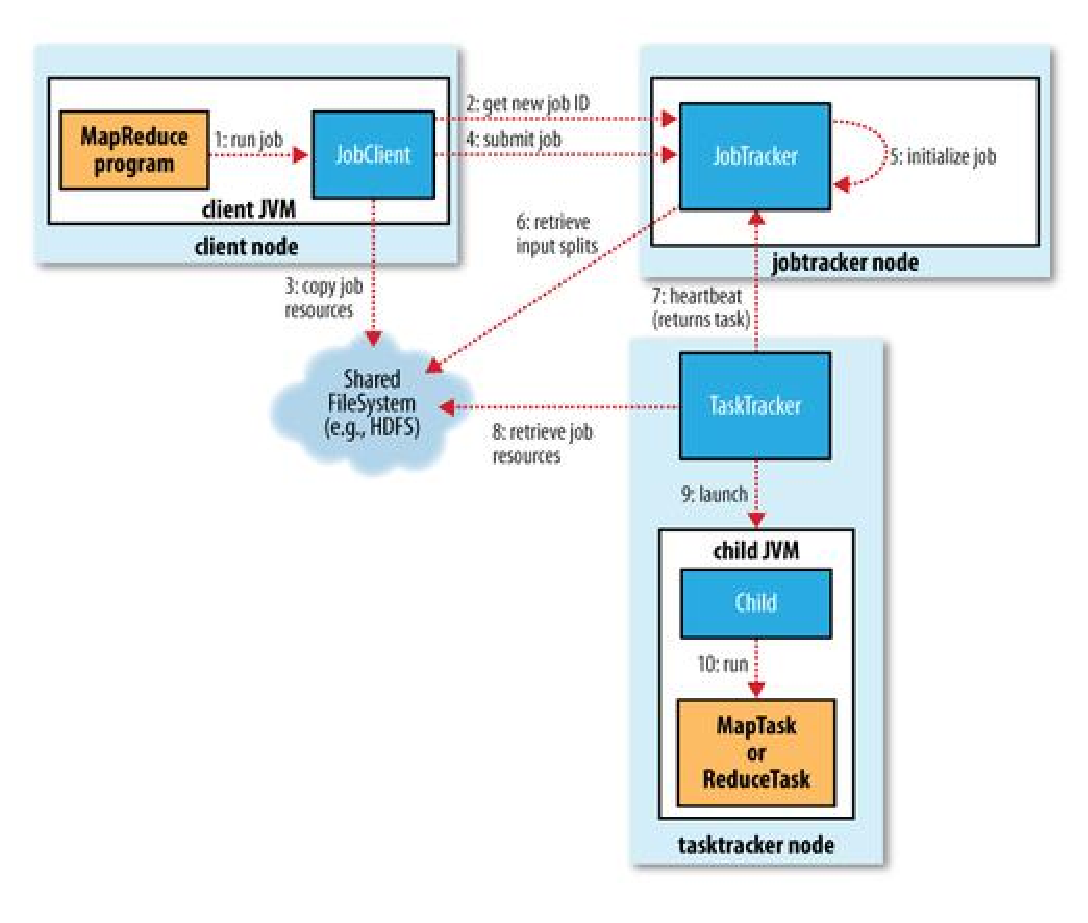
\includegraphics[width=8cm]{pics/mapred}}

\begin{figure*}[hbt]
\centerline{\includegraphics[width=12cm]{pics/hadoop}}
\caption{How Hadoop works}
\end{figure*}





\subsubsection{Pig: Graph-based workflow on Hadoop}
\subsubsection{Cascading}

\subsection{Scientific Workflow Systems}
\subsubsection{\textcolor{red2}{\bf{}Swift: Distributed parallel
    scripting}}
\bit
\w M.~Wilde, M.~Hategan, J.~M. Wozniak, B.~Clifford, D.~S. Katz, and I.~Foster.
\newblock Swift: A language for distributed parallel scripting.
\newblock {\em Parallel Computing}, 37(9):633--652, September 2011.
\w Some similarities to Hadoop, Pig.
\w A swift script consists of apps, where a \bb{app} is a script taking files as
    inputs and outputs.
\eit
\subsubsection{Kepler: Scientific workflow}
\subsection{Enterprise Workflow Systems}

\subsubsection{Activiti}
\subsubsection{Cascading}
\subsubsection{OSWorkflow}
 



\section{EVENT PROCESSING SYSTEMS}
\subsection{Event Publish/Subscribe Systems}
\bit
\w A.-M. Kermarrec and P.~Triantafillou.
\newblock {XL} peer-to-peer pub/sub systems.
\newblock {\em ACM Computing Surveys}, 46(2):16:1--16:45, November 2013.

\w A.~Carzaniga, D.~S. Rosenblum, and A.~L. Wolf.
\newblock Achieving expressiveness and scalability in an {I}nternet-scale event
  notification service.
\newblock In {\em Proceedings of the 19~th ACM Symposium on Principles of
  Distributed Computing (PODC'00)}, July 2000.
\eit

\subsection{Active Databases}
\bit
\w 
\eit

\subsection{CEP (Complex Event Processing)}
\bit
\w G.~Cugola and A.~Margara.
\newblock Processing flows of information: From data stream to complex event
  processing.
\newblock {\em ACM Computing Surveys}, 44(3):1--69, June 2012.

\w O.~Etzion and P.~Niblett.
\newblock {\em Event Processing in Action}.
\newblock Manning Publications Co., 2011.
\eit


\subsubsection{Esper}
\subsubsection{Oracle CEP}


\section{MESSAGING SYSTEMS}
\subsection{Enterprise Integration Patterns}
\bit
\w Hohpe and Woolf.
\newblock {\em Enterprise Integration Patterns: Designing, Building, and
  Deploying Messaging Solutions}.
\newblock Addison-Wesley, Reading, MA, 2003.
\eit
\subsection{JMS (Java Message Service)}
\bit
\w JSR 343:
\newblock Java message service 2.0, May 2013.
\eit
\bit
\w \bb{typical JMS Client}
\ben
\w use JNDI to find a \bb{ConnectionFactory} object
\w use JNDI to find one or more \bb{Destination} objects
\w use \bb{ConnectionFactory} to create a JMS \bb{Connection} with message
delivery inhibited
\w use \bb{Connection} to create one or more JMS \bb{Session}s
\w use \bb{Session} and \bb{Destination}s to create \bb{MessageProducer}s and
\bb{MessageConsumer}s
\w tell the \bb{Connection} to start delivery of messages
\een
\eit

\subsection{Messaging Protocols}
\subsubsection{AMQP}
\bit
\w obsolete -> see ZMQ
\eit
\subsubsection{\textcolor{red2}{\bf{}ZMQ}}
\bit
\w implemented in ZeroMQ system
\eit

\subsubsection{\textcolor{red2}{\bf{}MQTT}}
\bit
\w \bb{servers}: centralized cloud-based servers (bad idea) (e.g. Xively,
Device Cloud, ...)
\w \bb{brokers}: RabbitMQ, eMQTT (Erlang MQTT broker), ActiveMQ, ...
\w \bb{client libraries}: binding in different languages
(C/C++/Clojure/Erlang/Java/Objective-C/Perl/PHP/Ruby/...) for different
device platforms (Arduino/mbed/Nanode/Netduino/...) allows to use MQTT
protocol
\eit
\subsection{Message Queues}
\subsubsection{ActiveMQ}
\subsubsection{RabbitMQ}
\subsubsection{\textcolor{red2}{\bf{}ZeroMQ (also, Crossroads I/O)}}
\bit
\w P.~Hintjens.
\newblock {\em {ZeroMQ}}.
\newblock O'Reilly \& Associates, 2013.
\eit

\begin{figure*}[hbt]
\centerline{\includegraphics[width=16cm]{pics/zmq21-classes}}
\caption{ZeroMQ 2.0 Classes}
\end{figure*}

\subsubsection{TIBCO}
\subsubsection{MSMQ (Microsoft Message Queueing)}
\subsubsection{Apache Camel}
\bit
\w provides integration framework through route building
\w adding tap to components
\eit

\subsection{ESB (Enterprise Service Bus)}
\bit
\w D.~A. Chappell.
\newblock {\em Enterprise Service Bus}.
\newblock O'Reilly \& Associates, 2004.

\w T.~Rademakers and J.~Dirksen.
\newblock {\em Open Source ESBs in Action}.
\newblock Manning Publications Co., 2009.

\eit

%\begin{figure*}[hbt]
\centerline{\includegraphics[width=8cm]{pics/esb-01}}
%\caption{Enterprise Service Bus}
%\end{figure*}


\subsubsection{OpenESB}
\subsubsection{Mule}
\subsubsection{Apache ServiceMix (incl. Apache Camel)}
\subsubsection{Apache Synapse}
\subsubsection{D-Bus}
\bit
\w \bb{asynchronous} message buss for {\em interprocess communication\/} that
forms the backbone of GNOME/KDE desktop
\w shared bus architecture
\w applications connect to a bus (identified by a \bb{socket address}) and can
either transmit a targeted message to another application on the bus, or
broadcast a signal to all bus members

\w \bb{D-Bus daemon}: all processes communicate via the \bb{D-Bus daemon},
which handles:
  \ben
  \w [(a)] message passing
  \w [(b)] name registration
  \een
\w \bb{types of buses}
  \bit
  \w \bb{system bus}: allows users to communicate with system-wide components
  (printer, bluetooth, H/W devices, etc.); \underline{shared by all users}
  \w \bb{session bus}: unique to the user (one session bus for each logged-in
  user); used for user's applications to communicate with each other
  \eit
\w for applications to adopt D-bus protocol, there are several libraries
(e.g. GDBUS, libdbus, etc.), which allows:
   \bit
   \w to send/receive D-bus messages
   \w marshalling/unmarshalling types from language's  type-system to D-bus type-system
   \eit
\eit

\centerline{\includegraphics[width=8cm]{pics/d-bus}}


\section{ENTERPRISE COMPUTING}
\subsection{Java EE}
\subsection{OSGI}
\bit
\w service platform that implements complete and dynamic \bb{component model}
for Java
\w components are in the form of \bb{bundles for deployment} -- remotely
installed, started, stopped, updated, and uninstalled
\w OSGI service gateway architecture:\\

\centerline{\includegraphics[width=5cm]{pics/osgi-01}}

\w Classification: OSGI\\

\centerline{\includegraphics[width=8cm]{pics/osgi-02}}

\eit

\subsection{SOA in General}
\begin{figure}[hbt]
\centerline{\includegraphics[width=8cm]{pics/soa}}
\caption{SOA Environment}
\end{figure}

\begin{figure}[hbt]
\centerline{\includegraphics[width=8cm]{pics/soa-platform}}
\caption{SOA Technology Platform}
\end{figure}



\section{PERVASIVE COMPUTING}
\subsection{Wireless Sensor Networks}
\bit
\w D.~Estrin, D.~Culler, K.~Pister, and G.~Sukhatme.
\newblock Connecting the physical world with pervasive networks.
\newblock {\em IEEE Pervasive Computing}, pages 59--69, Jan--Mar 2002.
\eit

\subsection{Operating Systems for Devices}
\subsubsection{TinyOS}
\bit
\w microthreaded OS with small size (200-400B)
%\w \bb{event propagation time}: $\sim$ 10bit memory copy
\w TinyOS = \bb{tiny scheduler + a graph of components}, where each {\em
  component\/} consists of four parts:
  \ben
  \w [(a)] a set of {\em command handlers}
  \w [(b)] a set of {\em event handlers}
  \w [(c)] an encapsulated fixed-size {\em frame\/}
  \w [(d)] a bundle of simple {\em tasks}
  \een
\w tasks, commands, handlers execute in the context of the \bb{frame} and
operate on its \bb{state}
  \bit
  \w \bb{frame}: 
  \w \bb{command}: nonblocking request made to lower-level components;
  command will deposit request parameters into its frame and conditionally
  post a task for later execution; it may also invoke lower commands, but it
  must not wait for long or indeterminate latency actions to
  take place; a command must provide feedback to its caller 
  by returning status indicating whether it was successful or
  not, e.g., buffer overrun.

  \w \bb{event handler}: invoked to deal with {\em hardware events\/}, either
  directly or indirectly 
  \w \bb{task}: primary work performed atomically (i.e. run to completion),
  though can be preempted by events; 
     \ben
     \w call lower-level commands
     \w signal higher-level events
     \w schedule other tasks within a component
     \een
  \w \bb{task scheduler}:
  \eit
\eit
\subsubsection{Mote}

\subsubsection{ArdOS for Arduino}

\subsection{Database Systems for Devices}
\subsubsection{TinyDB}

\subsection{Programming Languages for Devices}
\subsubsection{nesC}
\bit
\w event-driven execution, flexible concurrency model, and component-oriented
application design 
\w supports {\em compile-time data race detection\/}
\w \bb{assumptions}:  
  \ben
  \w all resources are known statically
  \w rather than employing a general-purpose OS, applications are built from a
  suite of reusable system components coupled with application-specific code.
  \een
\eit

\section{ROBOTS, CARS, INDUSTRIAL AUTOMATION}
\subsection{CAN Bus}
\bit
\w 
\eit

\subsection{V2V}
\bit
\w 
\eit

\subsection{Robot Operating Systems}
\subsubsection{ROS}
\bit
\w \bb{ROS middleware}: the lowest level of ROS software stack -- offers a
message passing interface that provides means for inter-process communication 
   \bit
   \w \bb{publish/subscribe anonymous message passing}: asynchronous call
   \w \bb{recording and playback of messages}:
   \w \bb{request/response remote procedure calls}: for synchronous call -- \textcolor{red2}{preemptible}
    
   \w \bb{distributed parameter system}: global key-value store
   \eit
\w \textcolor{red2}{\bf Robot description language}
\w \bb{Robot-specific library}
\eit
\subsubsection{OPRoS}

\subsection{\textcolor{red2}{\bf{}OPC (Open Platform Communication)}}
\subsubsection{Overview}
OPC (\texttt{http://opcfoundation.org}) is the interoperability
standard for the secure and reliable exchange of data in the industrial
automation space and in other industries. It is platform independent and
ensures the seamless flow of information among devices from multiple
vendors. The OPC Foundation is responsible for the development and maintenance
of this standard.

\subsubsection{OPC UA (Unified Architecture)}
The OPC Unified Architecture (UA), released in 2008, is a platform independent
service-oriented architecture that integrates all the functionality of the
individual OPC Classic specifications into one extensible framework. 

This multi-layered approach accomplishes the original design specification
goals of: 
\bit
\w \bb{Functional equivalence}: all COM OPC Classic specifications are mapped
to UA 
\w \bb{Platform independence}: from an embedded micro-controller to
cloud-based infrastructure 
\w \bb{Secure}: encryption, authentication, and auditing
\w \bb{Extensible}: ability to add new features without affecting existing
applications 
\w \bb{Comprehensive information modeling}: for defining complex information
\eit

\paragraph{Functional Equivalence}
Building on the success of OPC Classic, OPC UA was designed to enhance and
surpass the capabilities of the OPC Classic specifications. OPC UA is
functionally equivalent to OPC Classic, yet capable of much more:
\bit
\w \bb{Discovery}: find the availability of OPC Servers on local PCs and/or networks
\w \bb{Address space}: all data is represented hierarchically (e.g. files and
folders) allowing for simple and complex structures to be discovered and
utilized by OPC Clients 
\w \bb{On-demand}: read and write data/information based on access-permissions
\w \bb{Subscriptions}: monitor data/information and report-by-exception when values change based on a client's criteria
\w \bb{Events}: notify important information based on client's criteria
\w \bb{Methods}: clients can execute programs, etc. based on methods defined
on the server
\eit
Integration between OPC UA products and OPC Classic products is easily
accomplished with COM/Proxy wrappers that are available in the download
section. 

\paragraph{Platform Independence}
Given the wide array of available hardware platforms and operating systems,
platform independence is essential. OPC UA functions on any of the following
and more: 
\bit
\w \bb{Hardware platforms}: traditional PC hardware, cloud-based servers,
PLCs, micro-controllers (ARM etc.) 
\w \bb{Operating Systems}: Microsoft Windows, Apple OSX, Android, or any
distribution of Linux, etc. 
\eit
OPC UA provides the necessary infrastructure for interoperability across the
enterprise, from machine-to-machine, machine-to-enterprise and everything
in-between. 
\paragraph{Security}
One of the most important considerations in choosing a technology is security. OPC UA is firewall-friendly while addressing security concerns by providing a suite of controls:
\bit
\w \bb{Transport}: numerous protocols are defined providing options such as
the ultra-fast OPC-binary transport or the more universally compatible
SOAP-HTTPS, for example 
\w \bb{Session Encryption}: messages are transmitted securely at 128 or 256
bit encryption levels
\w \bb{Message Signing}: messages are received exactly as they were sent
\w \bb{Sequenced Packets}: exposure to message replay attacks is eliminated with sequencing
\w \bb{Authentication}: each UA client and server is identified through OpenSSL certificates providing control over which applications and systems are permitted to connect with each other
\w \bb{User Control}: applications can require users to authenticate (login credentials, certificate, etc.) and can further restrict and enhance their capabilities with access rights and address-space ``views''
\w \bb{Auditing}: activities by user and/or system are logged providing an access audit trail
\eit
\paragraph{Extensible}
The multi-layered architecture of OPC UA provides a ``future proof''
framework. Innovative technologies and methodologies such as new transport
protocols, security algorithms, encoding standards, or application-services
can be incorporated into OPC UA while maintaining backwards compatibility for
existing products. UA products built today will work with the products of
tomorrow. 

\subsubsection{OPC Classic}
\bit
\w \bb{OPC Data Access (OPC DA)}:
The OPC DA specification defines the exchange of data including values, time and quality information.

\w \bb{OPC Alarms \& Events (OPC A\&E)}:
The OPC A\&E specification defines the exchange of alarm and event type message
information, as well as variable states and state management. 

\w \bb{OPC Historical Data Access (OPC HDA)}:
The OPC HDA specification defines query methods and analytics that may be
applied to historical, time-stamped data.
\eit


\section{DIGITAL SYSTEMS}
\subsection{Hardware Description Languages}
\subsubsection{Verilog}
\bit
\w IEEE~Std 1364-2001.
\newblock {IEEE Standard for Verilog Hardware Description Language}, 2005.
\eit
\subsubsection{Esterel}

\subsection{\textcolor{red2}{\bf{}Asynchronous Circuit Synthesis}}
\subsubsection{Phillips handshake circuits}
\subsubsection{BALSA}
\subsubsection{Petrify} 

\section{VIRTUALIZATION}
\subsection{Software Defined Networking (SDN)}
\subsubsection{Summary}
\bit
\w a.k.a. Network Virtualization (NV)
\w provides access to the forwarding plane of the network switch
\w OLD: packet arrives $\ra$ routing table lookup $\ra$ automatically
forwarded
\w NEW: with SDN installed on routers and switches, users can see flow table
and software-configure the network layout and traffic flow
   \bit
   \w e.g. netadmin can control the priority of packet switches (video packet
   preferred over emails
   \eit
\eit
\subsubsection{\textcolor{red2}{\bf{}OpenFlow}}

\subsection{Software Defined Storage}
\bit
\w a.k.a. Storage Virtualization (SV)
\eit
\subsubsection{NetApp}

\subsection{Software Defined Data Center}
\subsection{Software Defined Radio}

\section{SOFTWARE ARCHITECTURE AND PARADIGMS}
\subsection{Event-Based Programming Model}
\subsubsection{JavaScript}
\subsubsection{Twisted}
\subsubsection{X-Windows}

\subsection{\textcolor{red2}{\bf{}Continuations}}
\subsection{\textcolor{red2}{\bf{}Coroutines}}
\bit
\w \textcolor{blue2}{D.~Beazley.
\newblock A curious course on coroutines and concurrency.
\newblock {\texttt{}http://dabeaz.com/coroutines}, 2010.}
\w After all, talking distributed applications are coroutines.
\eit

\subsection{\textcolor{red2}{\bf{}Reactor/Proactor Design Pattern}}
\subsubsection{C10K problem}
\verb+http://www.kegel.com/c10k.html+
\subsubsection{C libevent}
\subsubsection{Python gevent}
\subsubsection{Akka I/O module}
\subsubsection{Boost.asio}
\subsubsection{Akka: Reactive stream}
\centerline{\includegraphics[width=8cm]{pics/akka-reactive-streams}}


\subsection{Aspect-oriented Programming}
\bit
\w cross-cutting concerns.
\w it's just making function calls ``hookable''; event generation when function
call begins and ends
\w NOTE: AOP was proposed by Kiczales, the inventor of Meta-Object Protocol
(CommonLoops), which explains much of the philosophy of AOP
\eit

\subsection{I/O systems}
\subsubsection{Java IO and NIO}
\subsubsection{C++ Streams I/O}
\bit
\w A \bb{stream} is either 
  \ben
  \w a standard stream such as \bb{cout}, \bb{cin}, and \bb{cerr}, or
  \w one created over a {\em file\/} or {\em device\/}
  \een
\w \bb{buffered stream} is a stream where {\em buffering\/} is enabled; 
\w \bb{buffering} has following benefits:
  \ben
  \w allows to cope with speed mismatch between producer and consumer
  \w allows producer to be nonblocking
   (no need to wait until the value is consumed)
  \een

\[ \xymatrix@-1.3pc {
&\mbox{\tt{}ios\_base} &\\
&\mbox{\tt{}basic\_ios<>} \ar[u]&\\
\mbox{\tt{}basic\_istream} \ar[ur] & & 
\mbox{\tt{}basic\_ostream} \ar[ul] \\
&\mbox{\tt{}basic\_iostream} \ar[ur]\ar[ul]&\\
}
\]


\w \bb{C++ output streams}
\bit
\w \bb{ostream} converts ``values of various types'' into \bb{sequences of
  characters} (or \bb{byte sequence}) 
\eit
\eit

\subsection{Telepathy: Instant messaging}
\bit
\w ``communications as a service'' (c.f. ``printing as a service'' -- each
application don't need to implement printing functionality; it can just use
printing service)
\w abstracting ``communication'' outside of an application
\w \bb{ConnectionManager}: one for each service (e.g. IRC, SIP, XMPP, etc.)
\w \bb{AccountManager}: for storing user's communication accounts and
establishing a connection to  each account via the appropriate connectino
manager when requested
\w \bb{ChannelDispatcher}:  listens for incoming channels signaled by each
ConnectinoManager and dispatch them to clients that indicate their ability to
handle that type of Channel (such as text, voice, video, file transfer,
tubes) 
  \bit
  \w also provides a service so that applications can request outgoing
  channels and have them handled locally by the appropriate client
  \eit
\w \bb{Telepathy clients}
\w \bb{Connection}
  \bit
  \w A \bb{Connection} will contain multiple \bb{Channel}s
  \w \bb{Channel}: the mechanism through which the communications are carried
  out (e.g. IM conversion, file transfer, voice or video call)
  \eit
\w {How Telepathy uses D-Bus}
  \bit
  \w every \bb{service} publishes a \bb{object path}, like
  \verb+org/freedesktop/Telepathy/AccntMgr+
  \w A service implements multiple \bb{interfaces}
    \bit
    \w a interface is strictly namespaced, like
    \verb+org.freedesktop.DBus.properties+ or \verb+oftT.connection+
    \w a interface provides \bb{methods}, \bb{signals}, or
    \bb{\underline{properties} that you can call/listen-to/request}
    \eit
  \w \bb{publishing D-Bus object} (= service registration)
    \bit
    \w add new (object-path, object) pair to the map of (object-path, object)
    pairs 
    \eit
  \w interfaces, methods, signals, properties are detailed in \bb{XML-based IDL}
     \bit
     \w can be used to generate stubs/wrappers and language bindings
     \eit
  \eit
\eit


\section{EXAMPLE SYSTEMS}
\subsection{Communication Protocols}
Some are \bb{request-response}-type of protocols while others are
\bb{publish-subscribe}-type of protocols. We need both.
\subsubsection{HTTP}
\subsubsection{RESTful HTTP}
\subsubsection{CoAP}
\subsubsection{MQTT}
\subsubsection{AMQP}
\subsubsection{AMQP-based DDS}
\subsubsection{SSI}
\subsubsection{XMPP}
\subsubsection{SSI}


\subsection{Protocol Standards Organization}
\subsubsection{\textcolor{red2}{OASIS}}

\subsection{Middleware}
\subsubsection{\textcolor{red2}{\textbf{}Qualcomm AllJoyn}}
\bit
\w \bb{Allseen Alliance}: Qualcomm, Microsoft, LG, Haier, Panasonic, Sharp,
       Technicolor, Silicon Image
\eit
\subsubsection{\textcolor{red2}{\textbf{}Open Interconnect Consortium}}
\bit
\w Intel, Samsung, Atmel, Broadcom, Dell, Wind River
\eit
\subsubsection{\textcolor{red2}{\textbf{}Thread Group}}
\bit
\w Google Nest Labs, ARM, Freescasle, Samsung, Yale Security, Silicon Labs
\eit



\subsubsection{Apple HomeKit}



\subsubsection{Google Glass}
\bit
\w \textcolor{blue2}{\bf\texttt{https://developers.google.com/glass/}}
\w Voice command: ``Get direction to San Francisco''
\begin{alltt}
  // navigation_trigger.xml
  \textbf{<trigger command="GET_DIRECTIONS_TO">
    <constraints
      network="true"
    />
    <input />
  </trigger>}
\end{alltt}

\begin{alltt}
  // AndroidManifest.xml
  <activity android:name=
            "NavigationActivity" />
    ...
    <intent-filter>
      <action android:name=
       "com.google.android.glass.
            action.VOICE_TRIGGER"/>
    </intent-filter>
    <meta-data
      android:name=
        "com.google.android.
             glass.action.VoiceTrigger"
      android:resource=
        "@xml/navigation_trigger"/>
  </activity>
\end{alltt}

\eit
\subsubsection{Google Fit}
\subsubsection{Google Nest}

\subsubsection{\textcolor{red2}{\bf{}Samsung SmartThings}}
\bit
\w platform for \textcolor{red2}{\bb{Open Physical Graph}}
\w cloud-based now, hub-based later
\w users create apps (to be executed in Cloud) using \bb{Groovy language}
\w layers:
  \ben
  \w \bb{Presentation layer (IPHONE)}: U/I in Web/Mobile applications
  \w \bb{Reactor layer (CLOUD)}: SmartApps \& SmartServices
  \w \bb{Device abstraction layer (CLOUD)}: Devices \& Capabilities
  \w \bb{Connectivity layer (CLOUD/DEVICE)}: Cloud Connectivity \& Device
primitives 
  \w \bb{Capability layer (DEVICE)}: Devices
  \een
\eit

\subsubsection{\textcolor{red2}{\bf{}Electric Imp}}
\bit
\w WiFi/Cortex M3
\w 128KB RAM (64KB for user code)
\w \bb{imp vs device}
  \bit
  \w \bb{imp}: hardware unit (imp card) which brings WiFi Internet
  connectivity and intelligence to a project
  \w \bb{device}: unique entity that combines an imp and other hardware
  component. 
  \eit
\w \bb{Squirrel language}
\w \bb{Imp IDE (web-based)}
   \bit
   \w \bb{Model}: each ``application''
   \w turn on device: will connect itself to cloud
   \w write code in Squirrel
   \w \bb{build and run}: will deploy code to device
   \eit
\eit

\subsubsection{\textcolor{red2}{\bf{}Zonoff}}


\subsection{Prototyping Boards}
\subsubsection{Arduino}
\bit
\w Atmel Atmega MCU
\eit
\subsubsection{Raspberry Pi}
\subsubsection{TI Beaglebone}
\subsubsection{Intel Galileo}
\subsubsection{Spark Core}
\bit
\w \texttt{http://spark.hackster.io}
\w 32-bit ARM CPU
\w 2MB flash memory
\w supports wireless deployment of code
\eit

\subsection{Devices}
\subsubsection{\textcolor{red2}{\bf{}Beacon}}
\subsubsection{Fitbit}
\bit
\w TI: MSP430F261T low-power MCU
\w Nordic: nRF24AP1 proprietary 2.4GHz RF chip with ANT low-power protocol
\w Freescale: MMA7341L 3-axis MEMS accelerometer
\eit
\subsubsection{Google Nest}
\subsubsection{Tagg GPS Pet Tracker}
\subsubsection{Aria weight scale}

\subsection{Misc systems}
\subsubsection{DIoTY.co}
\bit 
\w a cloud based platform to help you experiment faster with your IoT
projects.  
\w 
DIoTY currently provides you with two services, 
  \bit
  \w an MQTT broker 
  \w a Node-RED development tool.
  \eit
\w \bb{MQ Telemetry Transport (MQTT)}: lightweight broker-based
publish/subscribe messaging protocol.  MQTT was originally developed by IBM
but is currently standardized by OASIS and is both free and royalty free.  It
is rapidly becoming one of the standards for IoT/M2M.   
  \bit
  \w Clients (sensors, mobile apps,...) connect to a broker.
   \w Clients communicate by sending and receiving messages to/from the
broker.  
   For the broker, a messages is just a chuck of data.
  \w A client publishes a message to a topic (ego: /home/livingroom/temperature).
  \w A client can subscribe to many topics.  It will then start receiving all
messages send to those topic(s).
  \eit
\w As you can easily see, an MQTT broker as provided by DIoTY can remove the need to run your own web server at home.  Your sensors publish to the MQTT broker, your mobile app subscribes to the topics of interest and you're done... 

\w Node-RED is a visual tool for wiring the internet of things.  Node-RED is a creation of IBM emerging technologies, open source licensed under Apache 2.0.

\w With the Node-RED tool provided by DIoTY you can subscribe and publish to the MQTT broker.  You can alter the messages by applying functions to it (eg: subscribe to /home/livingroom/temperature/c ; convert the temperature from Celsius to Fahrenheit and then publish again to the topic /home/livingroom/temperature/f ). 

\w You can also interact over other protocols like http, websockets,... to retreive for example weather information from the bbc website and push it to your mobile application. 

\w Finally, with the twitter node, building your own twittering house becomes
as easy as pie.
\eit


%\bibliographystyle{plain}\bibliography{bib/mac,bib/compsys,bib/softsys,bib/digital,bib/formal,bib/theory,bib/algo,bib/pl,bib/misc}\nocite{Carbone06}
\end{document}

% LocalWords:  Birrell ACM IEEE Verilog compsys softsys Cheoljoo Jeong Cormen
%%  LocalWords:  Ashenhurst Leiserson Rivest Aho Sethi Ullman Saltzer Raynal
%%  LocalWords:  Kaashoek Kaufmann Verlag Agha Owicki Wobber SRC Henning CCS
%%  LocalWords:  CORBA Synchronizers Awerbuch Lamport Milner Hennessy Leeuwen
%%  LocalWords:  nondeterminism Parrow CSP Hoare Brookes polyadic Petri algo
%%  LocalWords:  Murata logics Pnueli Workflow Kermarrec Triantafillou Hohpe
%%  LocalWords:  Hintjens ZeroMQ O'Reilly ESB Rademakers Dirksen ESBs CEP IoT
%%  LocalWords:  Cugola Margara Etzion Niblett SOA et al Attiya Technion th
%%  LocalWords:  Karger Lewin Panigrahy Sussman Appel POPL Stoy Stratchey Lud
%%  LocalWords:  OOPSLA Bovet Cesati Ghemawat Gobioff Leung Google SOSP OSDI
%%  LocalWords:  workflow MapReduce Stoica Balakrishnan lookup SIGCOMM Shavit
%%  LocalWords:  Herlihy Amador Lazowska Littlefield Reuter Kauffman Chaib nd
%%  LocalWords:  Draa Dignum scher Altintas Jaeger Zhao kepler Carzaniga PODC
%%  LocalWords:  Rosenblum nternet JSR Chappell Dataflow Kahn IFIP Harel LFP
%%  LocalWords:  Statecharts Kushilevitz Reification SIGPLAN Abadi Cardelli
%%  LocalWords:  dRuby Scala Abramsky Gabbay Maibaum Automata Modelling Isard
%%  LocalWords:  Untimed Arvind ZigBee Mullender Gelernter toplas Lampson DNS
%%  LocalWords:  Prabhakaran Wieder Talwar LDAP JNDI NDS subcontext namespace
%%  LocalWords:  filesystem API javax aming SPI JDNI Surtani Infinispan MPI
%%  LocalWords:  OpenMP Cao Das Akka tuple tuples SystemVerilog Aglets Tcl Yu
%%  LocalWords:  D'Agents ObjectSpace IKV JavaSpace SwarmLinda TuCSoN Miloji
%%  LocalWords:  Douglis Finkel harlotte Paindaveine Zhou der Aalst Hee Budiu
%%  LocalWords:  Hollingsworth Runtime Fetterly SIGOPS EuroSys JVM mixin msg
% LocalWords:  GetSum Erlang shmem Pid rr rrd rru LOTOS Manas de SDL Holzmann
% LocalWords:  GFS Gnutella DHT UUID IIOP hostname TCP DCOM RMI Jini JMM akka
% LocalWords:  JavaSpaces javaSpaces Pthreads microkernel scala ActorRef WS
% LocalWords:  Typesafe BPEL ws bpel XPDL XLANG WWF CDL Desc Mendling Halfner
% LocalWords:  workflows LNCS Carbone Kohei Nobuko Yoshida CHOReOS multi SV
% LocalWords:  async priori Rossbach runtime Hadoop Hategan Katz Activiti JMS
% LocalWords:  OSWorkflow Esper ConnectionFactory MessageProducer AMQP ZMQ EE
% LocalWords:  MessageConsumer MQTT Xively CLoud RabbitMQ eMQTT erlang TIBCO
% LocalWords:  ActiveMQ Arduino MSMQ Queueing OpenESB ServiceMix interprocess
% LocalWords:  KDE bluetooth GDBUS libdbus marshalling unmarshalling OSGI OPC
% LocalWords:  uninstalled Estrin Culler Pister Sukhatme TinyOS microthreaded
% LocalWords:  nonblocking ArdOS TinyDB nesC middleware preemptible OPRoS UA
% LocalWords:  PLCs OSX HTTPS OpenSSL login HDA Esterel VIRTUALIZATION SDN ur
% LocalWords:  Virtualization netadmin OpenFlow NetApp JavaScript Coroutines
% LocalWords:  Beazley coroutines Proactor libevent gevent asio hookable AOP
% LocalWords:  Kiczales invetor CommonLoops NIO cout cin cerr ios istream ul
% LocalWords:  ostream iostream ConnectionManager IRC XMPP AccountManager IM
% LocalWords:  connectino ChannelDispatcher ConnectinoManager namespaced oftT
% LocalWords:  IDL COAP Qualcomm AllJoyn Allseen Haier Samsung Atmel Broadcom
% LocalWords:  Freescasle HomeKit xml AndroidManifest NavigationActivity MCU
% LocalWords:  Atmega Beaglebone Fitbit MSP nRF GHz Freescale MMA MEMS Tagg
% LocalWords:  GPS DIoTY MQ standardised
